\section{Resultados}

Con el archivo con extensión \textit{.l} definido, lo que necesitamos hacer es generar como salida un fichero fuente en C llamado \textbf{lex.yy.c}, para ello hacemos lo siguiente en nuestra terminal:

\begin{lstlisting}
flex practice.l
\end{lstlisting}

Luego, compilamos y enlazamos con la librería \textit{-ll}:

\begin{lstlisting}
gcc lex.yy.c -ll
\end{lstlisting}

Finalmente, ejecutamos:

\begin{lstlisting}
./a.out
\end{lstlisting}

Una vez el fichero se este ejecutando nosotros podremos probar nuestras definiciones y reglas:

\begin{figure}[H]
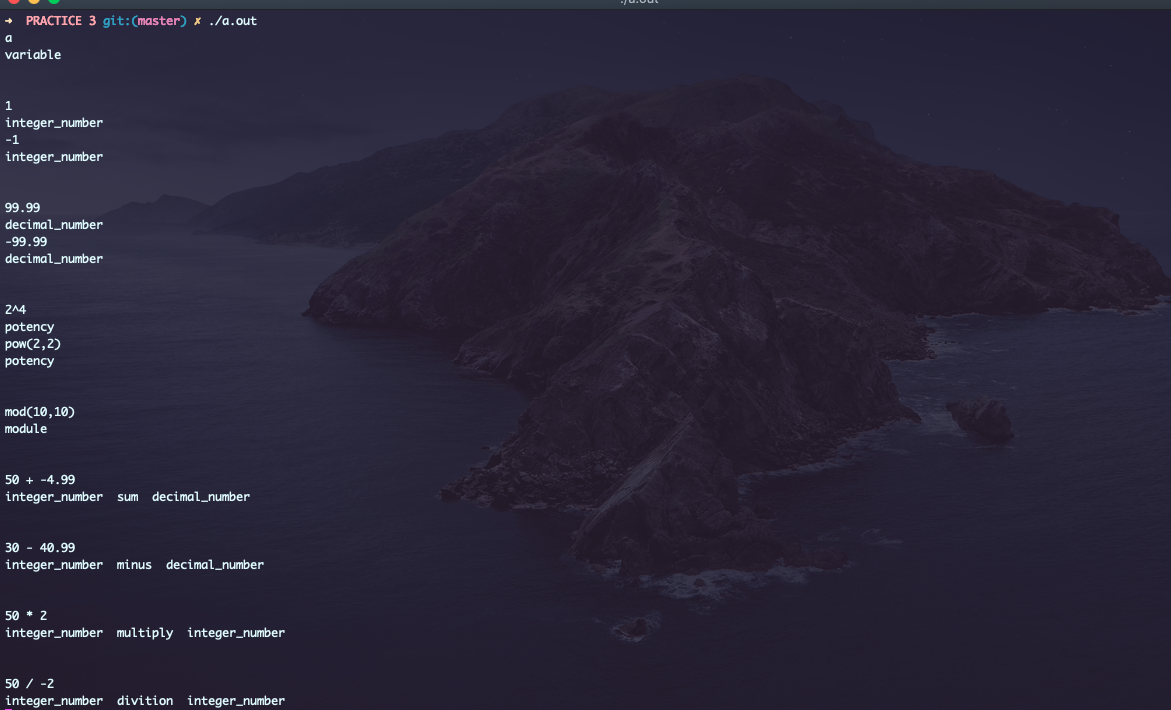
\includegraphics[width = 16.5cm, height = 12cm]{1.png}
\centering \linebreak \linebreak {\small Figure 1.0: Resultados del analizador léxico.}
\end{figure} 

\pagebreak